\documentclass[../Matt_Gebert_Honours_Thesis.tex]{subfiles}

\begin{document}
	
%	I will then describe the devices and measurements I have made in \cref{chap:fab&characterisation}. This will regard connections to devices, which allow the measurements I have perform, and the processes used to fabricate our devices. I have made graphene devices using lithography and evaporation methods, to create electrical contacts. I will also describe the oxides I have investigated in this chapter, and the methods I have used to transfer them.

	To create devices where we can measure the electronic properties referenced in \cref{sec:fet,sec:electronic_properties}, metalic contacts need to be added to the graphene to measure electronic flow through the device. 
	
	To do this, lithography can be used to create polymer structures that allow the deposition of desired material in 2D geometries. This process and the adjustements made for fabricating our devices are described in the sections below.

	\section{Lithography}\label{sec:lithography}
		Lithography typically consists of three steps.
		\begin{enumerate}
			\item Spin coating - covering your sample with a uniform layer of polymer.
			\item Exposure - exposing the polymer to light changes the chemical compounds and properties. This differentiates exposed areas to those unexposed.
			\item Developer solution - developer solution removes indended areas of photoresist to create structures.
		\end{enumerate}
		
	\subsection{Spin coating photoresists}\label{sec:resists}
		A spin coater is used to deposit thin films of materials. A vacuum is used to hold a sample horizontally on the spinner, before drops of photoresist are dropped onto the sample. The sample is then spun over sometime to achieve a uniform thickness of the photoresist, before baking on a hotplate occurs to set the sample.
		
		Photoresists vary in their spinning thickness, but also their exposure rates. Positive photoresists dissolve in developer when exposed to light, while negative photoresists dissolve if not exposed to light. We have only used positive photoresists, as we have primarily been creating structures for deposition, and not etching material (protect your sample, but remove everything else).
		
	\subsubsection{HMDS \& AZ-1512}
		Initially devices were fabricated using the AZ-1512 polymer, with the additional use of hexamethyldisilazane (HMDS) as an adhesion promoter between SiO$_2$ and AZ-1512. Devices were spun initially for 10 s at 1000 rpm, before being spun between 2000 and 3000 rpm for 30 s, per resist layer. This leaves a thickness of 1.7 $\mu$m to 1.39 $\mu$m \cite{az1500_series}.
		Devices were then baked at 100 $^\circ$C for 1 minute.
	
	\begin{figure}[H]\label{fig:spin_curve_AZ-1512}
		\centering
		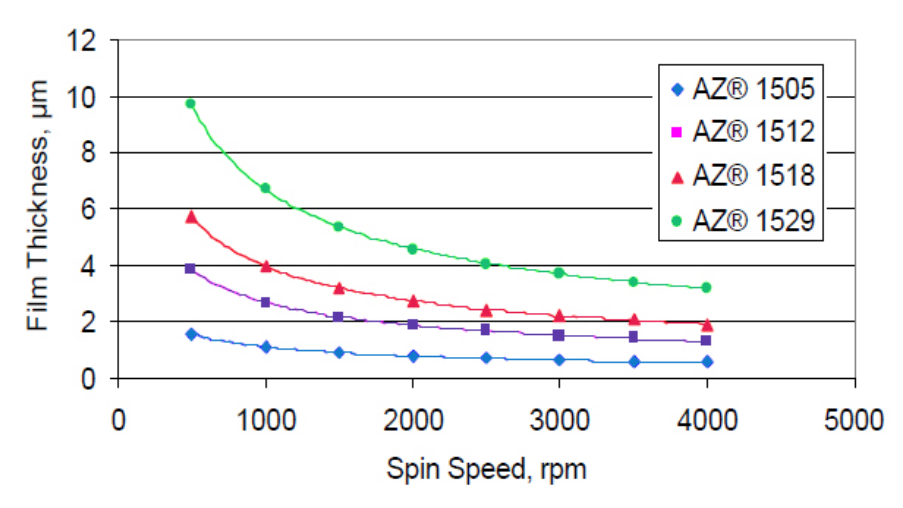
\includegraphics[width=0.7\textwidth]{chap2/az1512-spin-curve.png}
		\caption{Spin curve of AZ-1512 (Source: EMD Performance Materials\cite{az1500_series_spincurve})}
	\end{figure}
	
	\subsubsection{Skin issues with HMDS}
	When using HMDS and AZ-1512 in conjunction, significant amounts of deposition remenants were found on samples as seen in . 
	
	\begin{figure}[H]
		\centering
		\begin{subfigure}[b]{0.3\textwidth}
			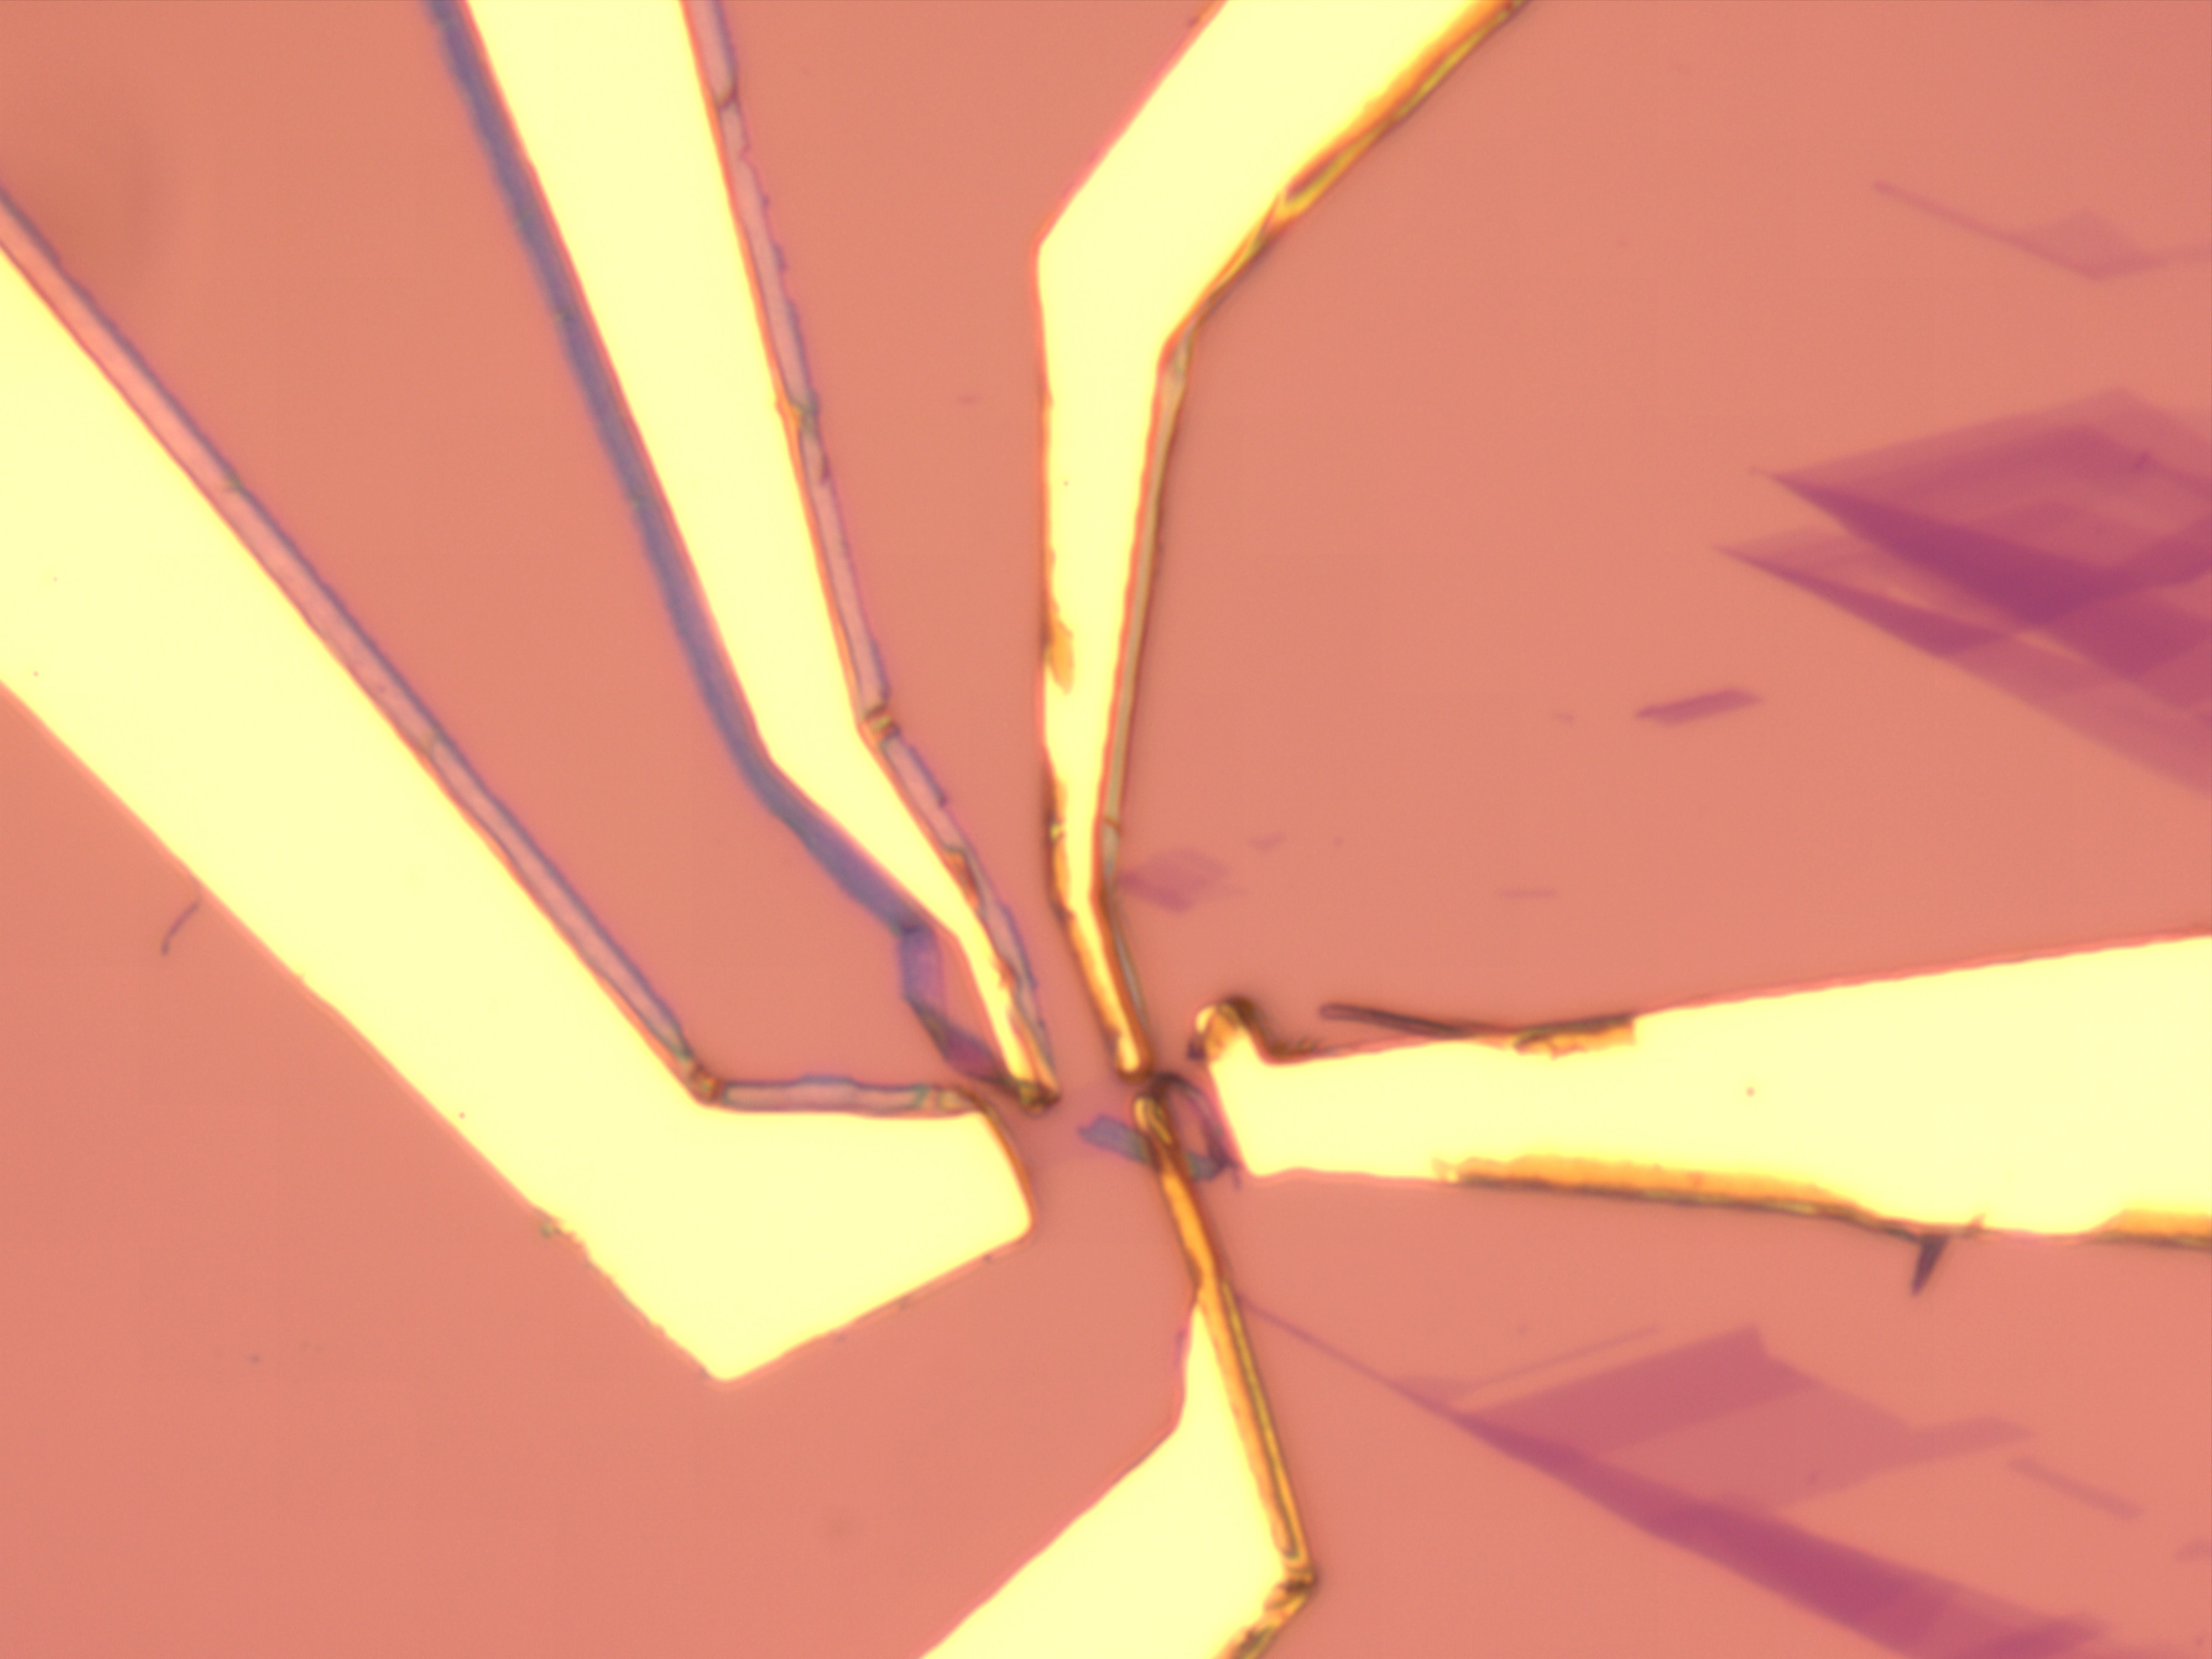
\includegraphics[width=\textwidth]{chap2/skins/Litho01_B07_WA1_F10_100x.jpg}
			\caption{After metal lift off}			
		\end{subfigure}
		\begin{subfigure}[b]{0.3\textwidth}
			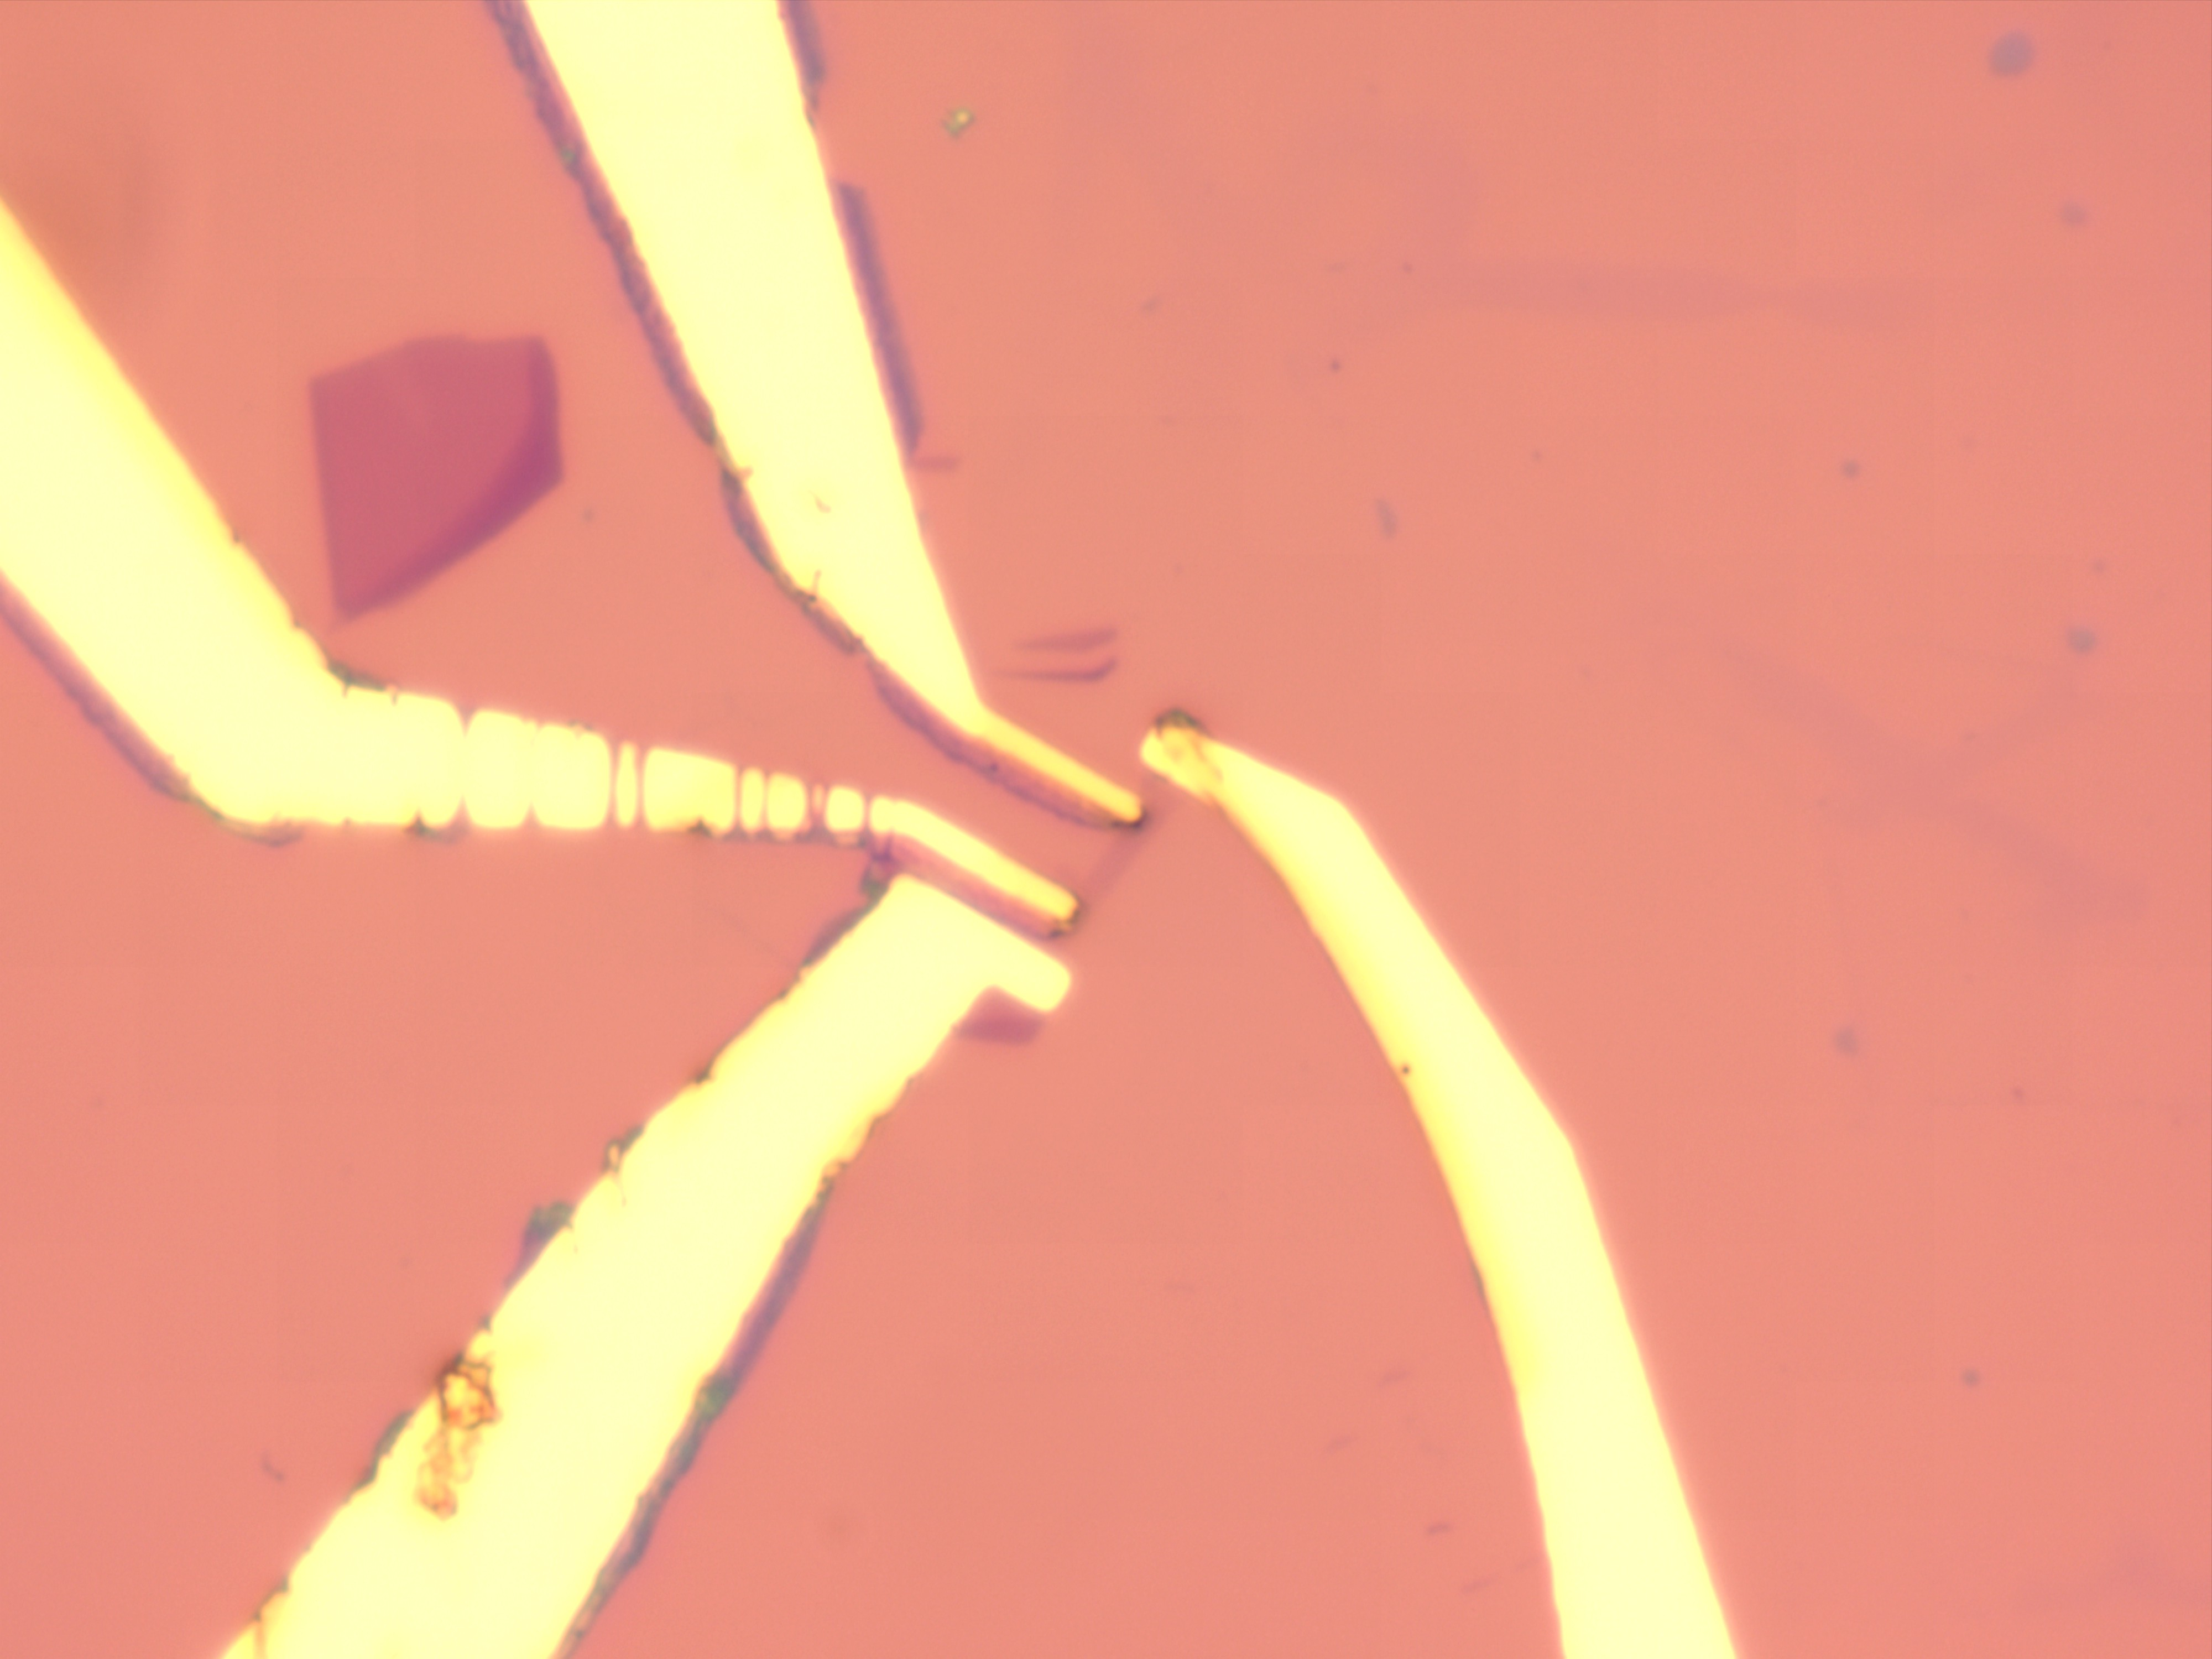
\includegraphics[width=\textwidth]{chap2/skins/1_100x.jpg}
			\subcaption{after 5s ultrasonication}
		\end{subfigure}
		\begin{subfigure}[b]{0.3\textwidth}
			\includegraphics[width=\textwidth]{chap2/skins/2_100x.jpg}
			\subcaption{after 10s ultrasonication}		
		\end{subfigure}
		\caption{Material remanants from lithography}\label{fig:lithography_skins}
		%TODO orientate images.
	\end{figure}
	
	Sometimes these could be cleaned off, through the use of ultrasonication, however this had a large risk of damaging the graphene, seen in \cref{fig:lithography_skins}.
	
	
	\begin{figure}[H]
		\centering
		\begin{subfigure}[b]{0.3\textwidth}
			\includegraphics[width=\textwidth]{chap2/US/2_100x.jpg}
			\caption{After metal lift off}			
		\end{subfigure}
		\begin{subfigure}[b]{0.3\textwidth}
			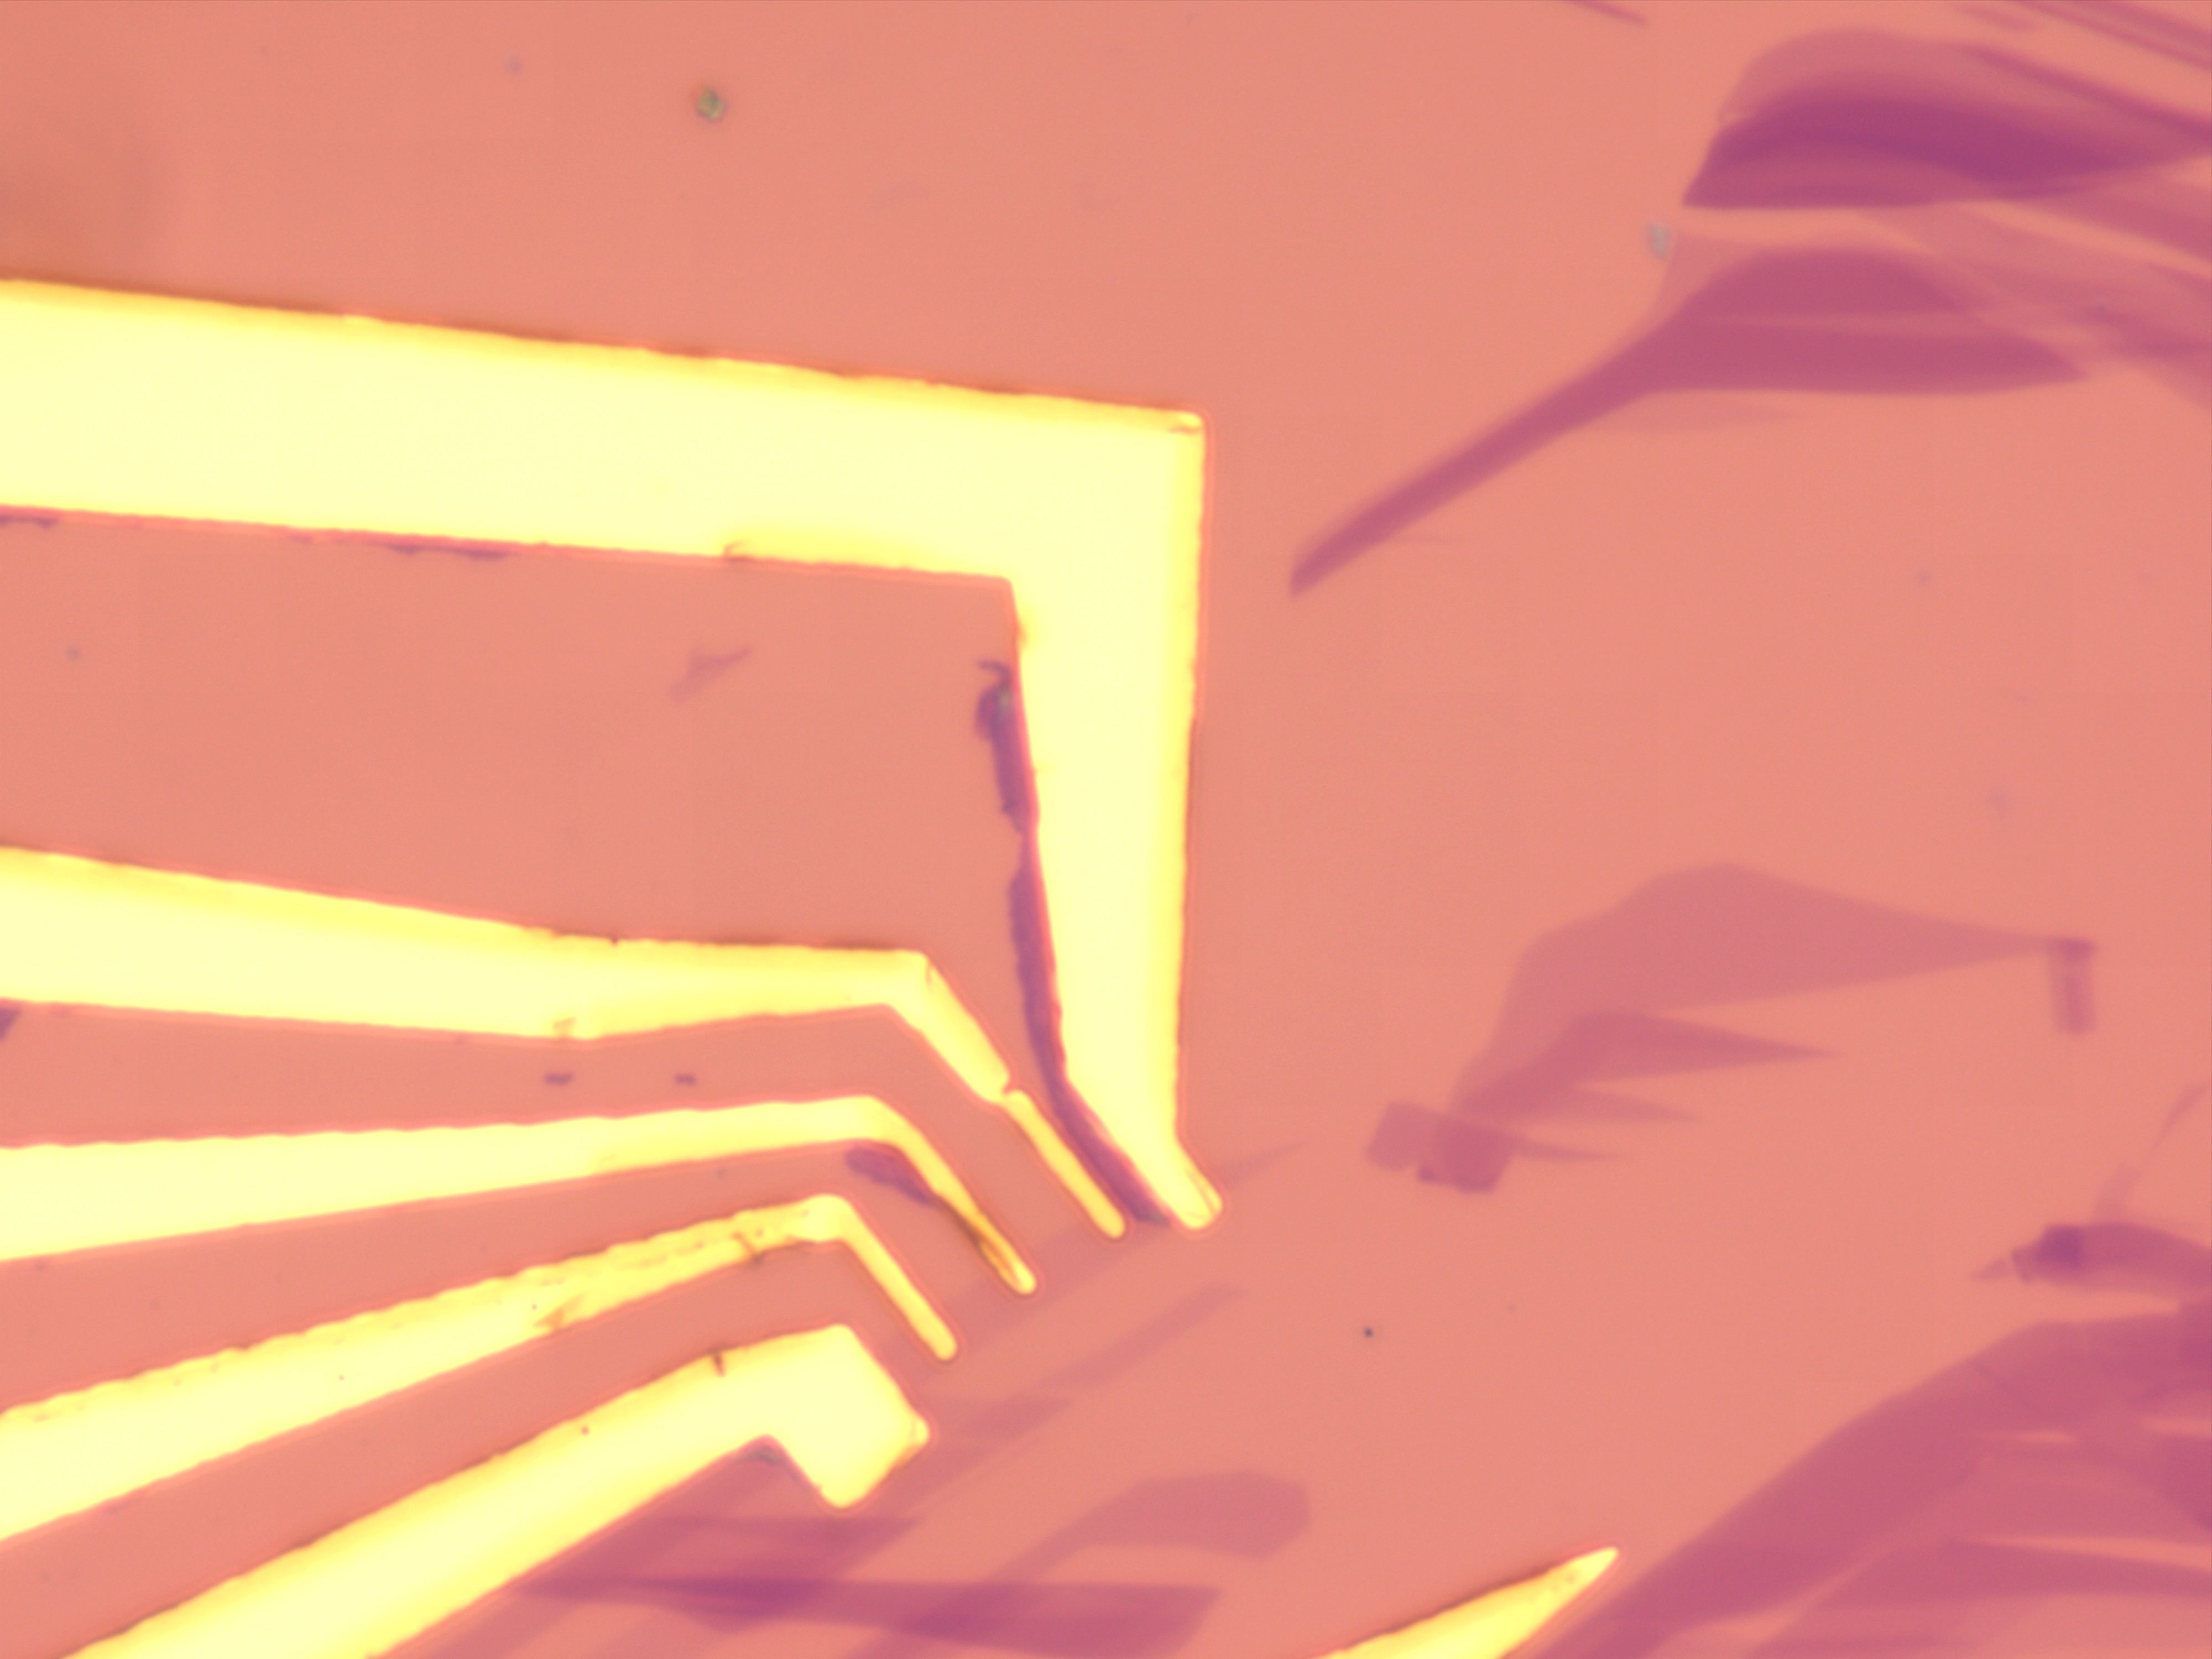
\includegraphics[width=\textwidth]{chap2/US/2_100x_after6sAcetoneUS.jpg}
			\subcaption{after 5s ultrasonication}
		\end{subfigure}
		\begin{subfigure}[b]{0.3\textwidth}
			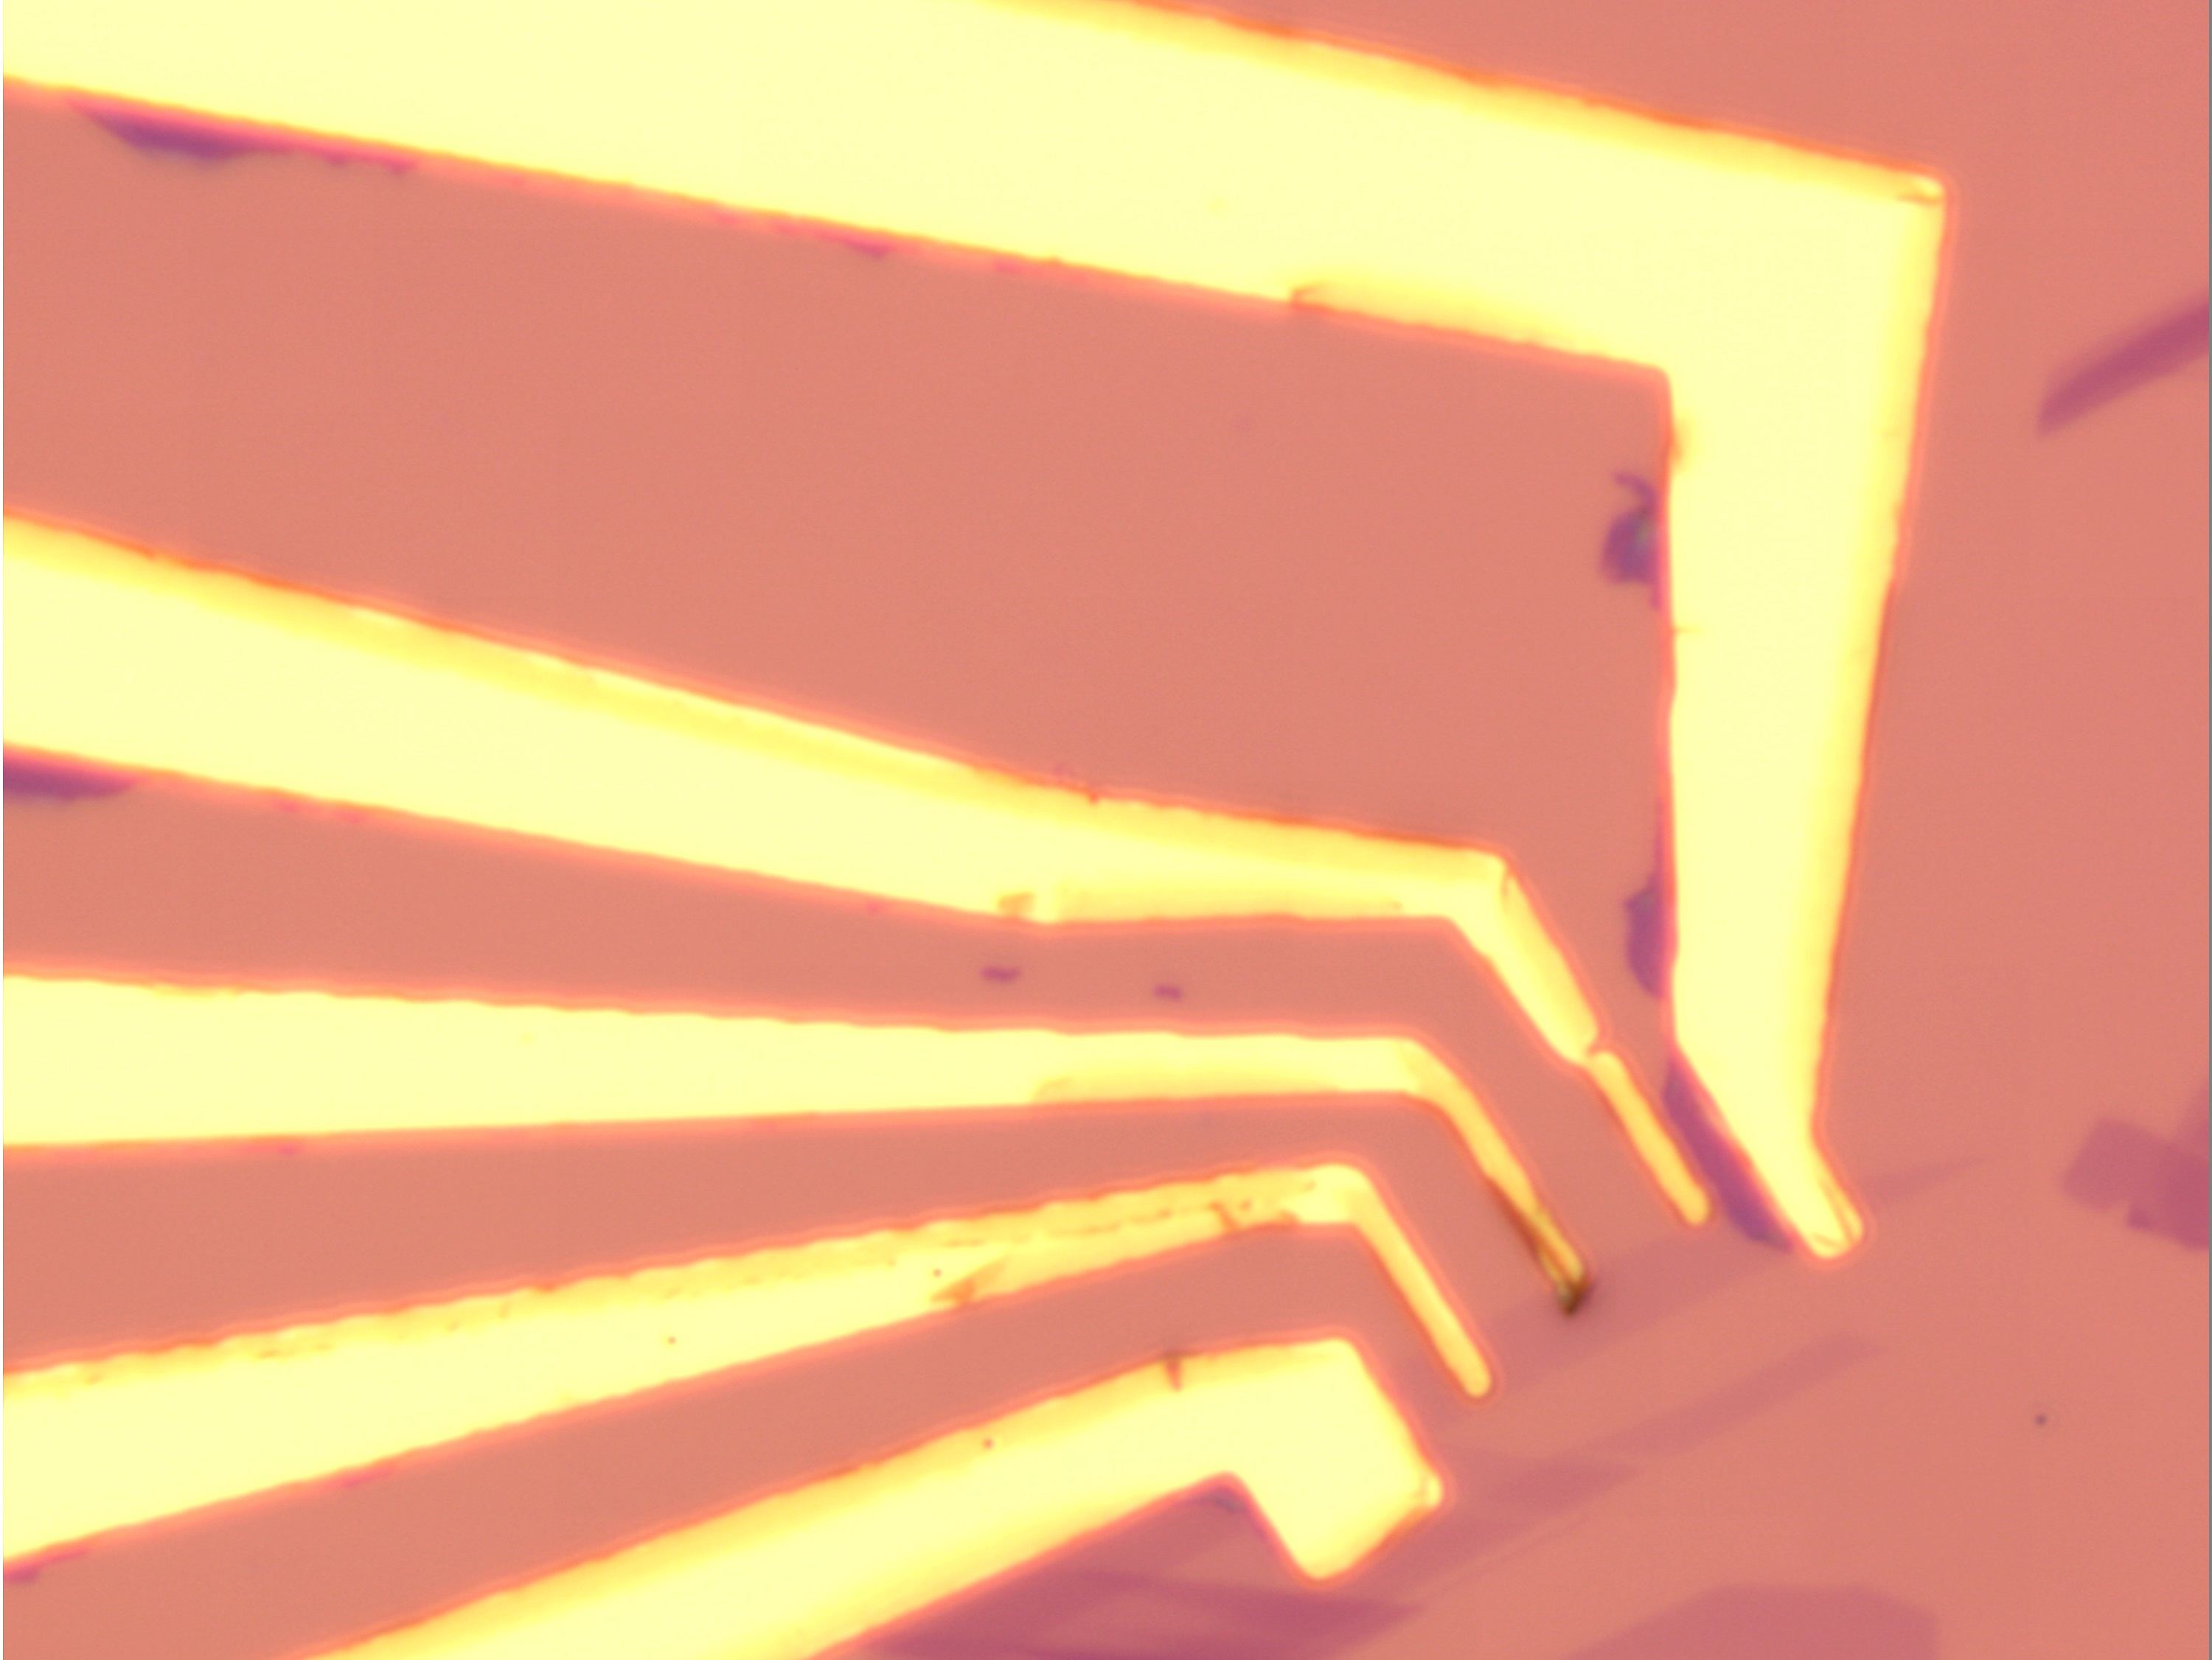
\includegraphics[width=\textwidth]{chap2/US/2_100x_after10sAcetoneUS.jpg}
			\subcaption{after 10s ultrasonication}		
		\end{subfigure}
		\caption{Material remanants from lithography}\label{fig:lithography_skins_us}
		%TODO orientate images.
	\end{figure}
	
	\subsubsection{LOR-1A \& AZ-1512}
	
	\subsection{Exposure}\label{sec:exposure}
		Photo mask writer
	
	\subsection{Developer}\label{sec:developer}
	
	\section{UV Ozone surface preparation}\label{sec:uv_ozone}
	
	\section{Deposition}\label{sec:deposition}
	
	\subsection{Oxide}
	
	\section{Lift-off}\label{}
	\subsection{Ultrasonication}
	
	\section{Oxide transfer}
	\subsection{Printing}
	\subsubsection{Al$_2$O$_3$}
	\subsubsection{SnO}
	\subsubsection{Bi$_2$O$_3$}
	
	\subsection{Smearing}
	\subsubsection{Ga$_2$O$_3$}
	
\end{document}